\documentclass[12pt]{article}


% --- math/fonts ---
\usepackage{amsmath,amssymb}
\usepackage{braket}
\usepackage[T1]{fontenc}
\usepackage{libertine}
\usepackage[utf8]{inputenc}

% --- graphics/tikz ---
\usepackage{tikz}
\usepackage{qcircuit}

% --- other stuff ---
\usepackage[margin=1in]{geometry}
\usepackage{pdfpages}
\usepackage{multicol}
\usepackage[shortlabels]{enumitem}
\usepackage{cancel}
\usepackage{graphicx}
\usepackage{float}
\usepackage{listings}
\usepackage{booktabs}
\lstset{
    language=Python,
    basicstyle=\ttfamily\footnotesize,
    keywordstyle=\bfseries,
    frame=single,
    breaklines=true,
    keepspaces=true,
    columns=fullflexible,
    showstringspaces=false
}
\let\epsilon\varepsilon
\usepackage{enumitem}
\setlist[enumerate]{label=\arabic*.}
\usepackage[authoryear,round]{natbib}
\usepackage[hidelinks]{hyperref}


\newcommand{\class}{CSCE883 Machine Learning}           
\newcommand{\examnum}{Homework 4}      
\newcommand{\examdate}{11/15/2026} % Add the submission date.        
\newcommand{\timelimit}{}             




\begin{document} 
\pagestyle{plain}
\thispagestyle{empty}

\noindent
\begin{tabular*}{\textwidth}{l @{\extracolsep{\fill}} r @{\extracolsep{6pt}} l}
 \textbf{\class} & \textbf{Name:} & \textit{Taylor Belcher}\\       
\textbf{\examnum} &&\\
\textbf{\examdate} &&\\
\end{tabular*}\\
\rule[2ex]{\textwidth}{2pt}
% ---

\begin{enumerate}
    \item \emph{(Question 1.)} Read the AlphaGo Paper. 
    \begin{enumerate}[a)]
        \item AlphaGo uses policy gradient reinforcement learning rather than Q-learning. For a given state, a policy network was trained starting with human expert choices and then improved with self-play. The policy network improves the distribution of possible moves to make in a given state by learning a better distribution of actions to take in that state. It is an attempt to answer the question, ``given this board state, where should we look for moves to make?'' Then they also train a value network that evaluates the expected outcome of a given state, training the network to better estimate that outcome without going the full depth of the game tree. The overall model uses a Monte Carlo Tree Search to apply the policy network and the value network to make a decision. The policy network decides where to search, the value network decides what is good. Both of these networks with MCTS help reduce the search space, the policy network reduces the breadth and the value network reduces the depth.
        \item The Go board itself is 19x19. The policy network represents the state using a $19\times19\times48$ stack of feature planes, including stone colors, liberties, capture size, and move history. The value network includes an additional binary plane recording whether the current player is black, giving it an input of $19\times19\times49$. Possible actions are legal moves in the current state, so either placing a stone at a legal empty intersection or passing the turn. Placements must satisfy the Go rules, including the ko restriction. This is a maximum of 19 x 19 + 1 = 362. Rewards are +1 for a terminal win, -1 for a terminal loss, and 0 for a non-terminal position, measured from the relevant player's perspective. Thus rewards come from the final game outcome rather than how good a particular move was.
        \item A policy network is trained on expert human moves to create a distribution of moves to consider in a given state. Then this distribution is improved further with self-play. The pseudocode is as follows:

        The first stage learns to predict the human move, and the second stage
        uses the final game outcome to improve the policy. The following is
        pseudocode adapted from the paper's Methods sections, ``Policy network:
        classification'' and ``Policy network: reinforcement learning.''

\par\medskip
\noindent\begin{minipage}{\linewidth}
\begin{lstlisting}[language={},mathescape=true]
Stage 1: Supervised learning from expert moves
    D = training pairs (board state s, expert move a)
    Augment D with the eight board rotations/reflections
    Initialize policy parameters $\sigma$
    Repeat for the supervised training steps:
        Sample a mini-batch B of 16 pairs from D
        g = 0
        For each (s, a) in B:
            g = g + $\nabla_\sigma \log p_\sigma(a \mid s)$
        $\sigma \leftarrow \sigma + (\alpha_{\rm SL}/16) g$

\end{lstlisting}
\end{minipage}
\par\medskip
\noindent\begin{minipage}{\linewidth}
\begin{lstlisting}[language={},mathescape=true]
Stage 2: Reinforcement learning by self-play
    Initialize $\rho \leftarrow \sigma$
    opponent_pool = {a frozen copy of $\sigma$}
    For iteration = 1, ..., 10000:
        Sample a frozen opponent from opponent_pool
        Play 128 games between $p_\rho$ and this opponent:
            Sample each move from the acting player's policy
            Save the states and moves until the game ends
            Assign each saved move its final outcome z:
                +1 if its player won, -1 if its player lost
        g = 0
        Replay the saved games:
            For each saved state s, move a, and outcome z:
                g = g + $(z-b(s))\nabla_\rho \log p_\rho(a \mid s)$
        $\rho \leftarrow \rho + (\alpha_{\rm RL}/128) g$
        If iteration is a multiple of 500:
            Add a frozen copy of $\rho$ to opponent_pool
\end{lstlisting}
\end{minipage}
\par\medskip

        Here $p_\sigma(a\mid s)$ is the supervised policy and
        $p_\rho(a\mid s)$ is the policy improved by reinforcement learning.
        The paper replays moves from both players to calculate the update,
        with $z$ measured from the player making that move's perspective.
        The baseline $b(s)$ is zero on the first pass through the training
        pipeline; on a second pass, the trained value network $v_\theta(s)$
        is used to reduce variance. Thus the reinforcement-learning step is
        REINFORCE with a baseline. A winning move sequence receives a
        positive outcome, while a losing sequence receives a negative one.
       
        \item The policy network reduces the breadth of the search by identifying promising moves, while the value network
        reduces the depth needed to evaluate a position. We need both because
        predicting which move to consider and predicting who will win from a
        position are different tasks. A likely move alone does not tell us the
        outcome of the game, and evaluating positions alone would still leave
        too many possible moves to search.

        The networks are connected during training. The supervised policy
        $p_\sigma$ is first trained on human moves, and the reinforcement-learning
        policy $p_\rho$ is initialized from it and improved with self-play.
        Self-play then provides state--outcome pairs $(s,z)$ to train the value
        network $v_\theta(s)$ to predict the expected outcome under the improved
        policy. Its objective is to minimize the mean squared error
        $\mathbb{E}[(v_\theta(s)-z)^2]$. The paper uses about 30 million positions,
        each from a different self-play game, to reduce overfitting caused by
        strongly correlated positions within the same game.

        When making a decision, AlphaGo combines the trained networks through
        MCTS. At an expanded node, the supervised policy supplies move priors
        $P(s,a)=p_\sigma(a\mid s)$, which guide exploration along with the search's
        current action values and visit counts. At a leaf position $s_L$, the
        value network's prediction is combined with the outcome $z_L$ of a
        rollout using a separate fast rollout policy:
        \[
            V(s_L)=(1-\lambda)v_\theta(s_L)+\lambda z_L.
        \]
        This evaluation is backed up through the search tree to update action
        values and visit counts. After the search, AlphaGo selects the most
        visited move at the root. The paper uses the supervised policy for
        these search priors because it worked better within MCTS than the
        stronger self-play policy. The self-play policy instead provides the
        games used to train the value network and the MCTS uses the trained network to choose a move. 

        
    \end{enumerate}

    \item \emph{(Question 2.)}
    I ran the three algorithms in the supplied
    \href{https://github.com/jordanlei/deep-reinforcement-learning-cartpole}{CartPole repository}:
    Deep Q-Network (DQN), REINFORCE, and Advantage Actor--Critic (A2C).
    The code and experiment outputs are in \texttt{Q2\_CartPole.ipynb}.
    Each algorithm was trained for 500 episodes for each of three random
    seeds (0, 1, and 2), giving 1,500 training episodes per algorithm.
    All methods used CartPole-v1, a discount factor of $\gamma=0.99$, and
    a finite horizon of 500 steps. The reward is $+1$ per step that the
    episode continues, so the maximum episode reward is 500.
    The learning rates were the repository's defaults: 0.001 for DQN and
    0.01 for REINFORCE and A2C. Training ran on the CPU.

    The notebook adapts the supplied code to Gymnasium, corrects the reward
    smoothing window, and gives DQN a separate frozen target network,
    updated every 40 episodes. The original DQN code uses the same object
    for its learner and target. These are results from the adapted code,
    rather than an exact execution of the original scripts.

    Figure~\ref{fig:q2-rewards} shows the episode rewards for all three
    algorithms. The thin lines show the individual seeds, the black line
    shows the mean across seeds of the trailing 20-episode average, and
    the shaded region shows one standard deviation across seeds.
    Figure~\ref{fig:q2-comparison} compares those smoothed learning curves.

    \begin{figure}[H]
        \centering
        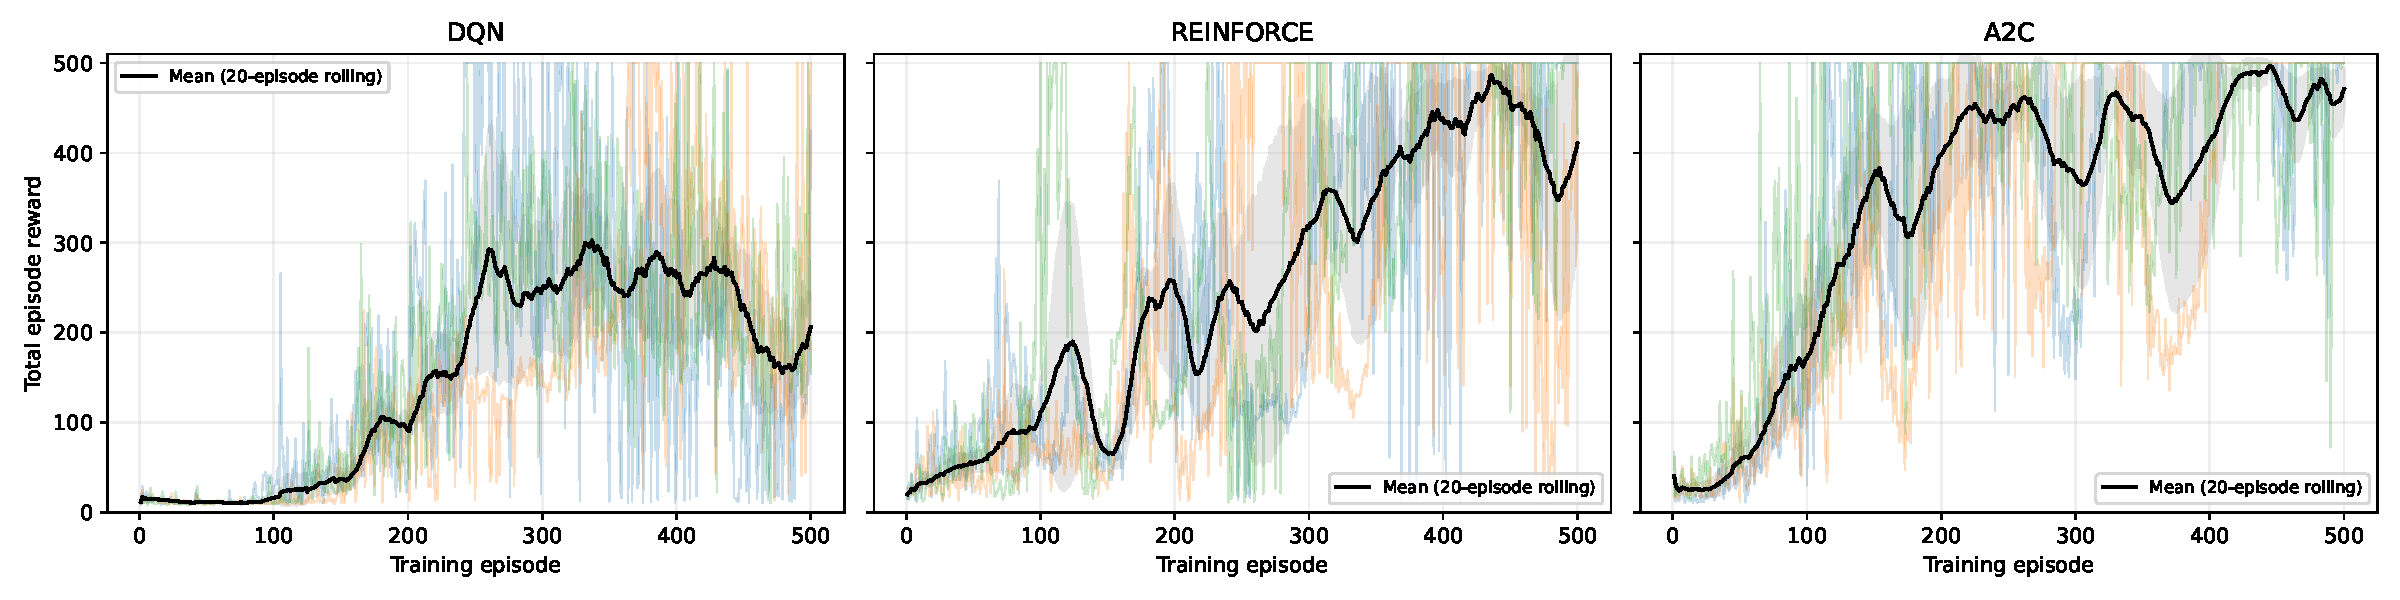
\includegraphics[width=\linewidth]{q2_results/20261115-155447/all_reward_curves.pdf}
        \caption{Episode rewards for DQN, REINFORCE, and A2C over 500 training episodes per seed.}
        \label{fig:q2-rewards}
    \end{figure}

    \begin{figure}[H]
        \centering
        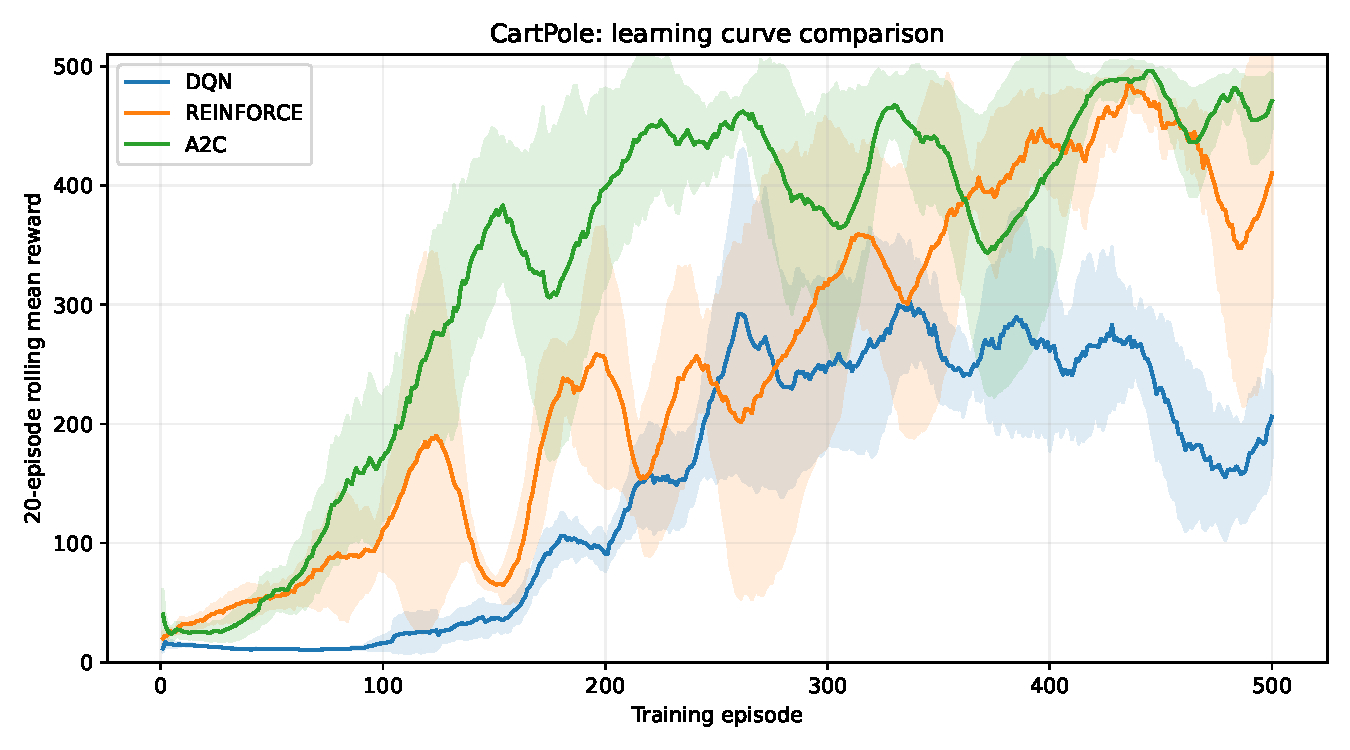
\includegraphics[width=0.9\linewidth]{q2_results/20261115-155447/comparison.pdf}
        \caption{Comparison of the trailing 20-episode mean rewards, averaged across three seeds. Shading shows one standard deviation across seeds.}
        \label{fig:q2-comparison}
    \end{figure}

    To compare final training performance, I averaged the rewards over
    the final 100 training episodes for each seed and then averaged these
    values across seeds. I also evaluated each trained model for 20 new
    episodes, giving 60 evaluation episodes per algorithm. Evaluation
    disables dropout and uses greedy actions for DQN and sampled actions
    for the two policy-based methods. Table~\ref{tab:q2-results} reports
    the results. The $\pm$ values are standard deviations of the three
    per-seed means, not confidence intervals.

    \begin{table}[H]
        \centering
        \small
        \begin{tabular}{lrrr}
            \toprule
            Algorithm & Whole-run mean & Final 100 mean & Evaluation mean \\
            \midrule
            DQN & 155.6 & $216.7\pm49.7$ & $152.1\pm43.0$ \\
            REINFORCE & 257.5 & $430.2\pm49.2$ & $500.0\pm0.0$ \\
            A2C & 345.6 & $472.3\pm18.0$ & $493.4\pm9.4$ \\
            \bottomrule
        \end{tabular}
        \caption{Mean episode rewards across three seeds. The whole-run mean uses all 500 training episodes per seed.}
        \label{tab:q2-results}
    \end{table}

    A2C had the best training performance in this experiment. It had the
    highest whole-run average reward and the highest final-100-episode
    average, with less variation across seeds than the other methods in
    that final window. However, REINFORCE had the best post-training
    evaluation performance: every evaluation episode reached the maximum
    reward of 500. A2C was close behind at 493.4, while DQN was substantially
    lower at 152.1. Thus A2C performed best by the training metric, while
    REINFORCE produced the best final evaluation results. These conclusions
    apply to this episode budget, these seeds, and the supplied
    hyperparameters; they do not establish that one algorithm is always
    better. Evaluation also differs from training because dropout and
    DQN's exploratory actions are disabled.

    \noindent\textit{AI-use disclosure for Question 2:}
    I used OpenAI's Codex assistant to prepare and adapt the supplied code
    into a Jupyter notebook and to summarize the saved results in LaTeX.
    I ran the training experiments locally.


    \item \emph{(Question 3.)}
    \begin{enumerate}[a)]
        \item % Your answer to 3(a).
        \item % Your answer to 3(b).
    \end{enumerate}

    \item \emph{(Question 4.)}
    % Your answer to Question 4.
\end{enumerate}

\end{document}
